\documentclass{resume}

\usepackage{hyperref}
\usepackage{fontawesome}
\usepackage{wasysym} 
\begin{document}

\fontfamily{ppl}\selectfont

\noindent
\begin{tabularx}{\linewidth}{@{}m{0.8\textwidth} m{0.2\textwidth}@{}}
{
    \Large{Kristof G. Herrmann} \newline
    \small{
        \clink{
            \href{mailto:kristof.herrmann@rwth-aachen.de}{kristof.herrmann@rwth-aachen.de} \textbf{·} 
            {\fontdimen2\font=0.75ex +49 151 2014 2005}
            \textbf{·} 
            {\fontdimen2\font=0.75ex Cologne, Germany}
        } 
        \begin{flushleft}
            \footnotesize Highly motivated \textbf{mathematician and developer} (IoT) with keen interest in complex problems. More than 2 years of experience in developing industrial software from shopfloor level to the cloud. Project management, requirements analysis, planning, testing and documentation.
        \end{flushleft}
    }
} & 
{
    \hfill
    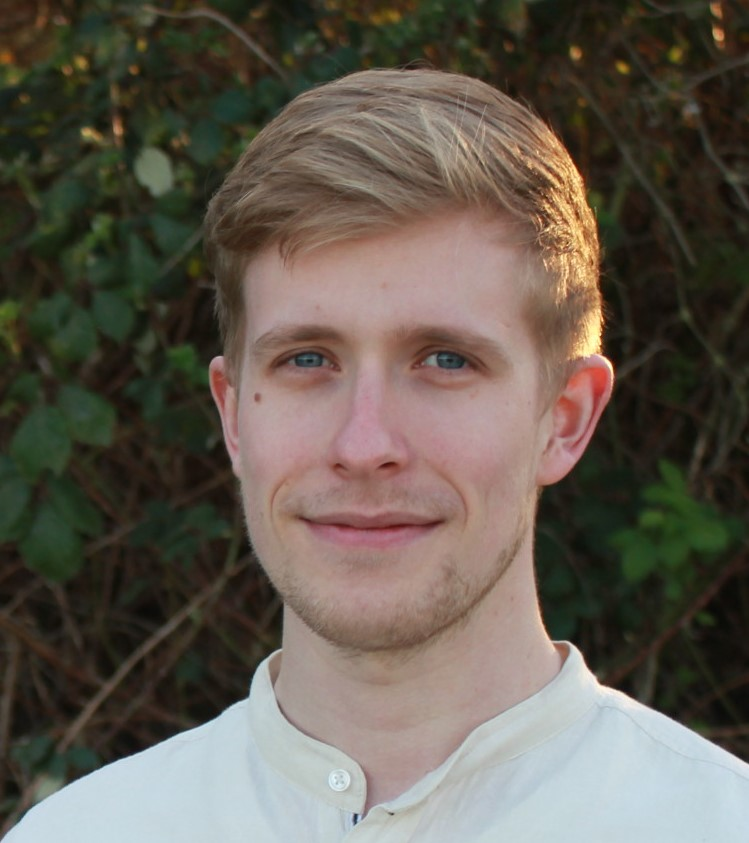
\includegraphics[width=2.7cm]{images/portrait.jpg}
}
\end{tabularx}
\vspace{-5mm}
\begin{center}
\small "I want to further improve my project management skills, take on responsibility and be part of an innovative team that creates digital solutions with real added value."
%\vspace{5mm}


\vspace{5mm} 
\begin{tabularx}{\linewidth}{@{}*{2}{X}@{}}
% left side %
{
    \csection{WORK EXPERIENCE}{\small
        \begin{itemize}
            % item 1 %
            \item \frcontent{Senseering GmbH}{Full Stack Software Engineer - Cologne}{
            Developer of a decentralized data sharing platform in the spirit of \href{https://www.bmwi.de/Redaktion/DE/Dossier/gaia-x.html}{GAIA-X}. Technical consultant IoT solutions.}{since April 2020}
             \item \frcontent{WZL der RWTH Aachen}{Working Student - Aachen}{Developer of a decentralized data sharing platform in the spirit of \href{https://www.bmwi.de/Redaktion/DE/Dossier/gaia-x.html}{GAIA-X} with a focus on Data Science.}{April 2019 - April 2020}
            \item \frcontent{PricewaterhouseCoopers GmbH}{Intern Business Intelligence - Düsseldorf}{Development of a planning tool for the maintenance and repair of vehicles for a large German transport service provider.}{October 2018 - Februar 2019}
            % item 2 %
            \item \frcontent{RWTH Aachen}{Tutor for higher mathematics - Aachen}{}{October 2015 - September 2018}
        \end{itemize}
    }
    \csection{EDUCATION}{\small
        \begin{itemize}
            % item 1 %
            \item \frcontent{M.Sc. Mathematics \footnotesize $\diameter$1.0}{Focus on partial differential equations. Field of application: computer science. Rheinisch-Westfälische Technische Hochschule Aachen }{}{Autumn 2017 - Autumn 2019}
            \item \frcontent{B.Sc. Mathematics \footnotesize $\diameter$1.8}{Focus on measure theory. Field of application: computer science. Rheinisch-Westfälische Technische Hochschule Aachen}{}{Autumn 2014 - Autumn 2017}
        \end{itemize}
    }
     \csection{AWARDS}{\small
        \begin{itemize}
            % item 1 %
            \item \frcontent{\href{https://www.spaicer.de/}{Springorum-Denkmünze} }{proRWTH - top 10\% of each faculty}{}{2020}
        \end{itemize}
    }
} 
% end left side %
& 
% right side %
{
    \csection{SKILLS}{\small
        \begin{itemize}
             \item \textbf{Programming languages \& Databases} \newline
            {\footnotesize Nodejs, Vue, Python, MySQL, Mongodb, InfluxDB, Elasticsearch, Redis}
            \item \textbf{Cloud \& Technologies} \newline
            {\footnotesize S3/Azure Blob Storage, EC2, CodeBuild, CodePipeline, CDN, ECS,ELK, Azure IoT Hub, Grafana, Docker, Portainer, Node Red, Github Actions, DynamoDB, AWS Cognito, KeyCloak, Auth0, IOTA, Nginx, httpd}
            \item \textbf{Mathematics} \newline
            {\footnotesize Partial differential equations, measure theory, numerical analysis, financial mathematics }
              \item \textbf{Languages} \newline
            {\footnotesize german, english}
        \end{itemize}
    }
    \csection{PROJECTS}{\small
        \begin{itemize}
            \item \frcontent{spaicer \clink{\href{https://www.spaicer.de/}{[spaicer.de]}}}{Scalable adaptive production systems through AI-based resilience optimization - Project responsibility. }{}{IoT, machine learning, AI}
            \item \frcontent{obsidian \clink{\href{https://github.com/Senseering/obsidian}{[Senseering/obsidian]}}}{A Nodejs based immutability layer for (industrial) data}{Release pending}{Nodejs, IOTA}
             \item \frcontent{MyDataEconomy \clink{\href{https://www.mydataeconomy.com}{[mydataeconomy.com]}}}{Decentralized IoT data sharing platform for sovereign data exchange.}{}{GAIA-X, Nodejs, Docker, IOTA, InfluxDB}
             \item \frcontent{Duck \clink{\href{https://arzelaascoii.github.io/UAVDocs}{[arzelaascoii.github.io/UAVDocs]}}}{Autonomous flying solar plane built from scratch.}{}{UAV, Ardupilot, ROS, Docusaurus}
        \end{itemize}
    }
    \vspace{5mm}
\begin{center}
\begin{tabularx}{\linewidth}{@{}*{3}{X}@{}}
\centering{\href{https://www.linkedin.com/in/kgherr}{ \Large  \faLinkedinSquare } }
&
\centering{ \href{https://github.com/ArzelaAscoIi}{\Large \faGithub } }
&{\hspace{13mm}\href{https://www.medium.com/@Kristof.herrmann}{\Large \faMedium }}
\\
\centering\small kgherr &
\centering\small ArzelaAscoIi  & 
\centering\small @Kristof.herrmann
\end{tabularx}

\end{center}
     
    
    %\csection{OTHER HIGHLIGHTS}{\small
    %%    \begin{itemize}
     %       \item {\footnotesize Gave talk on \textit{Achieving Rapid Response Times in Large Online Services} at Berkeley AMPLab Cloud.}
     %       \item {\footnotesize Led several teams across infrastructure, founded \textit{Google Brain} and was involved in hiring process.}
     %   \end{itemize}
    %}
    %\csection{HOBBIES \& INTERESTS}{\small
    %    \vspace{0.32cm}
    %    \begin{tabularx}{\linewidth}{@{}*{4}{>{\centering\arraybackslash}X}@{}}
    %%        {\centering
     %       
\includegraphics[width=0.8cm]{images/userexperience.png}
     %%       } &
       %     {\centering
        %    
\includegraphics[width=0.8cm]{images/lamp.png}
         %   } & 
         %   {\centering
        %    
\includegraphics[width=0.8cm]{images/healthcare.png}
    %        } &
     %       {\centering
     %       
\includegraphics[width=0.8cm]{images/cauldron.png}
     %       } \\
     %       {\footnotesize UI/UX} & {\footnotesize Problem Solving} & {\footnotesize Healthcare} & %{\footnotesize Open Source}
     %   \end{tabularx}
    %}
}
\end{tabularx}
\end{center}

\end{document}